\thispagestyle{empty}
%Layout and components including source, mirrors, lens design, beamsplitter
%details, detectors, and detector arrangement.
\subsection{Fresnel lens}
The physical constraints of installing a full-view imaging interferometer on
the H-1 heliac requires imaging lenses with focal lengths $\approx 600
- 800$mm and diameters (or cross-section thereof) $\approx
600$mm.
For typical construction materials such as polymethylpentene
(PMP, also known as TPX) ($n_{\rm PMP} = 1.465$) and high density
polyethylene ($n_{\rm HDPE} = 1.53$), radii of curvature of $300 -
400$mm are needed, resulting in extremely large centreline thicknesses and
attentuation.
To satisfy these constraints---and after initially evaluating imaging properties\cite{MAHON2011}---a Fresnel lens design was chosen.
The lens has been precision machined from a single piece of PMP.
\begin{figure}[htbp]
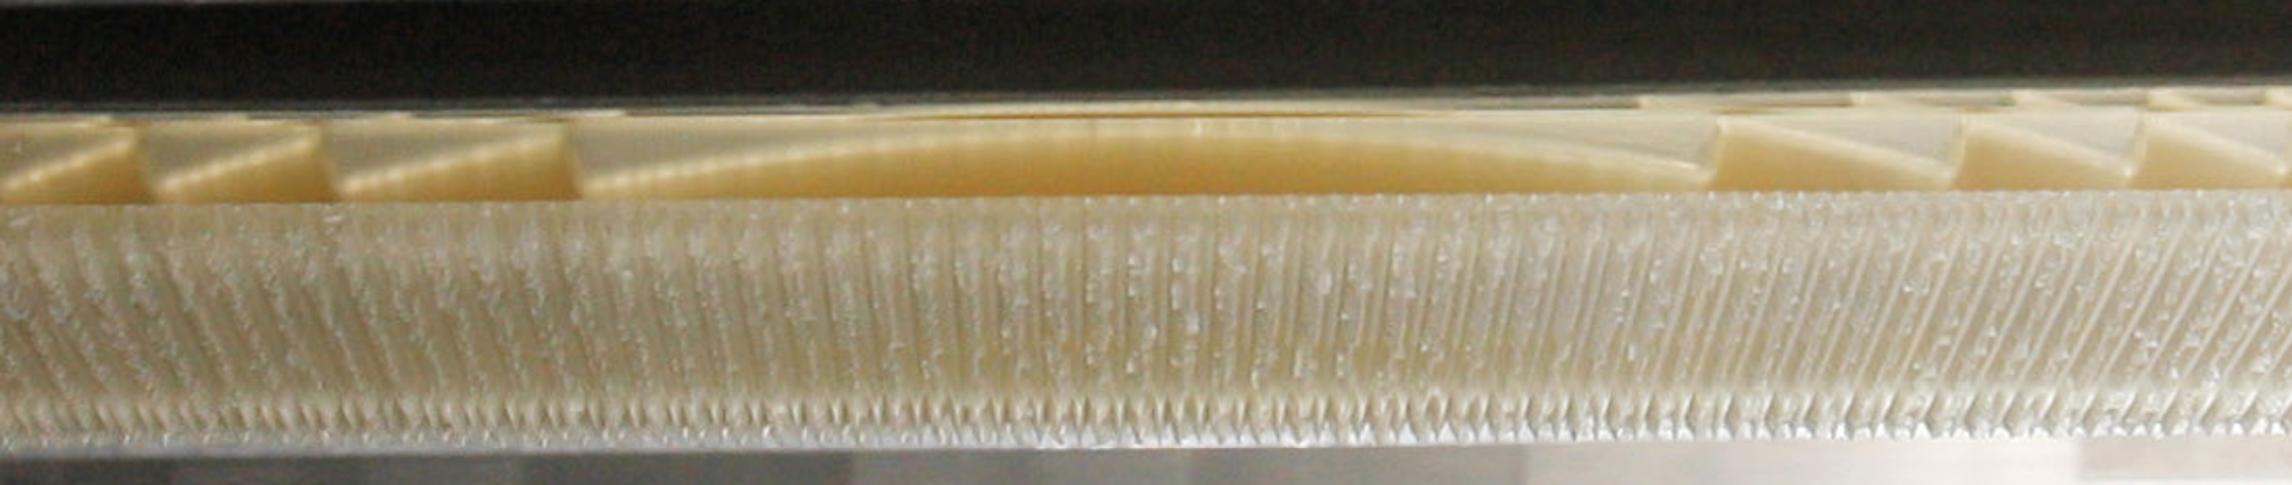
\includegraphics[width=\columnwidth]{figures/fresnel_lens_detail}
\caption{Detail of the centre portion of the cylindrical Fresnel lens,
  seen from the side. The pyramidally-textured surface machined into
  the plane side of the lens reduces reflection.}% See \S \ref{sec:antiref_techniques}.}
\label{fig:antiref_photo}
\end{figure}

\subsection{Free-wire Beamsplitter}
High performance beamsplitters in the millimeter-wave range can be
constructed using a grating approach with closely-spaced, thin,
conductive wire, though this can prove challenging for large aperture optics.
For $\lambda \gg r$ (the radius of the wire), the co-efficient of reflection of the grating is given by
\cite{CASEY1952, RENK1962}
\begin{equation}
R = 1 - \left[ \frac{2d}{\lambda} \ln (\frac{d}{2 \pi r}) \right] ^2
\label{eq:beamsplitter_trans}
\end{equation}
and absoprtion by
\begin{equation}
A = \frac{d}{\pi r} \left[ {\frac{c}{\sigma \lambda}} \right]
^{\frac{1}{2}} R
\label{eq:beamsplitter_abs}
\end{equation}
where $d$ is the wire spacing, $\sigma$ is conductivity of the wire,
and $c$ is the speed of light.
For tungsten wire with $r = 5$\ts{}$\mu$m, a wire separation $d =
70$\ts{}$\mu$m, and $\sigma = 1.89 \times 10^7$\ts{}S/m

Meeting the challenge of a large aperture beamsplitter required
support frames suitable to meet the tension from many, closely-spaced
wound wires together with a metal-working lathe sufficiently large to
wind the beamsplitter.
Two support frames were bolted together, back-to-back, mounted and
turned slowly on a suitable lathe, winding $\approx 4000$\ts{}m of
tungsten wire over the pair.
Wires are glued to the frame, a securing clamping frame is attached
and the wires along the coupled frames' edges are cut, separating the
two beamsplitters.

For an incident wave polarized perpendicular to the wires the
beamsplitter is nearly completely transparent while waves polarized
parrallel are partially transmitted and partially reflected.\cite[p.280]{MARCUVITZ1951}
Thus, for a wave launched with polarization at 45\degrees{} to
horizontal wires, the reflected wave will be nearly completely
horizontally polarized and the transmitted wave a mix of both vertical
and horizontal polarizations.
The second beamsplitter thus reflects the horizontally-polarized
`leaked' component of the wave transmitted from the first beamsplitter
and a beam dump is installed on the vertical support table to suppress
reflection of this wave back into the optical path.

\subsection{Quarter-wave Plate}
The optical layout and power efficiency of the interferometer design
is dependent on a suitably performing quarter-wave plate. Various designs
of form birefringent components exist\cite{VANVLIET81} allowing
flexibility in the design of a suitable wave plate. 

\subsection{Anti-reflection Techniques}
\label{sec:antiref_techniques}
Reducing the contribution of minor reflection cavities within the
optical layout to the final interferogram is a priority in improving
the reliability of the measurement of the phase shift in the probe arm
and, hence, the electron density measurements.
One technique to reduce these contributions is to tilt the optical
components from normal incidence such that the initial pass of the
beam through them is relatively undisturbed but subsequent
reflections, say from the next optical component, are reflected out of
the beam path.
The vacuum window-lens, shown in Figure \ref{fig:overview_schematic},
has such a tilt along the longtitudinal axis permanently integrated as
part of the lens design.
Other lenses, such as the imaging and detector focussing lenses, are
able to be rotated longtitudinally as part of their mounting system.
To further reduce unwanted reflections within the system a pyramidally
textured surface\cite{DEINEGA2010} is machined into the plane side
of each lens, as shown in Figure\ref{fig:antiref_photo}.
The pyramid peaks are spaced 2\ts{}mm apart with a peak-to-base depth
of 2.6\ts{}mm.
